\documentclass[mathserif]{beamer}

\setbeamertemplate{frametitle}[default][center]%Centers the frame title.
\setbeamertemplate{navigation symbols}{}%Removes navigation symbols.
\setbeamertemplate{footline}{\raisebox{5pt}{\makebox[\paperwidth]{\hfill\makebox[10pt]{\scriptsize\insertframenumber}}}}
\setbeamertemplate{caption}[numbered]

%\newcommand{\tth}   {\mbox{$\theta$}}
\newcommand{\thh}   {\mbox{$\theta$}}
\newcommand{\su}   {\mbox{$\sigma^2$}}
\newcommand{\so}   {\mbox{$\sigma_0^2$}}
\newcommand{\ko}   {\mbox{$\kappa_0$}}
\newcommand{\no}   {\mbox{$\nu_0$}}
\newcommand{\mo}   {\mbox{$\mu_0$}}
\newcommand{\ti}   {\mbox{$\tilde{x}$}}
\newcommand{\la}   {\mbox{$\lambda$}}
\newcommand{\bx}   {\mbox{$\bm{x}$}}
\newcommand{\bZ}   {\mbox{$\bm{Z}$}}
\newcommand{\bX}   {\mbox{$\bm{X}$}}
\newcommand{\bY}   {\mbox{$\bm{Y}$}}
\newcommand{\bA}   {\mbox{$\bm{A}$}}
\newcommand{\ba}   {\mbox{$\bm{a}$}}
\newcommand{\bb}   {\mbox{$\bm{b}$}}
\newcommand{\bt}   {\mbox{$\bm{t}$}}
\newcommand{\bz}   {\mbox{$\bm{z}$}}
\newcommand{\bw}   {\mbox{$\bm{w}$}}
\newcommand{\bbeta}   {\mbox{$\bm{\beta}$}}

\newcommand{\be}   {\mbox{$\bm{e}$}}
\newcommand{\bu}   {\mbox{$\bm{u}$}}
\newcommand{\bv}   {\mbox{$\bm{v}$}}
\newcommand{\sig}   {\mbox{$\Sigma$}}
\newcommand{\sigx}   {\mbox{$\Sigma_{XX}$}}
\newcommand{\sigxy}   {\mbox{$\Sigma_{XY}$}}
\newcommand{\tr}   {\mbox{$\text{tr}$}}
\newcommand{\ddet}   {\mbox{$\text{det}$}}
\newcommand\independent{\protect\mathpalette{\protect\independenT}{\perp}}
\def\independenT#1#2{\mathrel{\rlap{$#1#2$}\mkern2mu{#1#2}}}

\newcommand{\Expect}[1]{\ensuremath{\mathbf{E}\left[ #1 \right]}}
%\newcommand{\Var}[1]{\ensuremath{\mathrm{Var}\left[ #1 \right]}}
%\newcommand{\Cov}[1]{\ensuremath{\mathrm{Cov}\left[ #1 \right]}}
\newcommand{\MSE}{\ensuremath{\mathrm{MSE}}}
\newcommand{\RSS}{\ensuremath{\mathrm{RSS}}}
\newcommand{\Prob}[1]{\ensuremath{\mathrm{Pr}\left( #1 \right)}}
\newcommand{\ProbEst}[1]{\ensuremath{\widehat{\mathrm{Pr}}\left( #1 \right)}}
\DeclareMathOperator*{\argmin}{argmin} % thanks, wikipedia!
\DeclareMathOperator*{\argmax}{argmax} % thanks, wikipedia!
\DeclareMathOperator*{\sgn}{sgn} % thanks, wikipedia!

\newcommand{\lam}{\lambda}
\newcommand{\bmu}{\bm{\mu}}
%\newcommand{\bx}{\ensuremath{\mathbf{X}}}
\newcommand{\X}{\ensuremath{\mathbf{X}}}
\newcommand{\w}{\ensuremath{\mathbf{w}}}
\newcommand{\h}{\ensuremath{\mathbf{h}}}
\newcommand{\V}{\ensuremath{\mathbf{V}}}
%\newcommand{\tr}{\operatorname{tr}}

%\newcommand{\bx}{\ensuremath{\mathbf{X}}}
%\newcommand{\X}{\ensuremath{\mathbf{x}}}
%\newcommand{\w}{\ensuremath{\mathbf{w}}}
%\newcommand{\h}{\ensuremath{\mathbf{h}}}
%\newcommand{\V}{\ensuremath{\mathbf{v}}}
%\newcommand{\Cov}{\text{Cov}}
%\newcommand{\Var}{\text{Var}}

\DeclareMathOperator{\var}{Var}
\DeclareMathOperator{\cov}{Cov}
\newcommand{\Var}[1]{\ensuremath{\mathrm{Var}\left[ #1 \right]}}
\newcommand{\Cov}[1]{\ensuremath{\mathrm{Cov}\left[ #1 \right]}}


\newcommand{\indep}{\rotatebox{90}{\ensuremath{\models}}}
\newcommand{\notindep}{\not\hspace{-.05in}\indep}







\usepackage{float}
\floatstyle{boxed}
\newfloat{code}{tp}{code}
\floatname{code}{Code Example}
\newcommand{\tth}   {\mbox{$\theta$}}
\newcommand{\thh}   {\mbox{$\theta$}}
\newcommand{\su}   {\mbox{$\sigma^2$}}
\newcommand{\so}   {\mbox{$\sigma_0^2$}}
\newcommand{\ko}   {\mbox{$\kappa_0$}}
\newcommand{\no}   {\mbox{$\nu_0$}}
\newcommand{\mo}   {\mbox{$\mu_0$}}
\newcommand{\ti}   {\mbox{$\tilde{x}$}}
\newcommand{\la}   {\mbox{$\lambda$}}
\newcommand{\bx}   {\mbox{$\bm{x}$}}
\newcommand{\bZ}   {\mbox{$\bm{Z}$}}
\newcommand{\bX}   {\mbox{$\bm{X}$}}
\newcommand{\bY}   {\mbox{$\bm{Y}$}}
\newcommand{\bA}   {\mbox{$\bm{A}$}}
\newcommand{\ba}   {\mbox{$\bm{a}$}}
\newcommand{\bb}   {\mbox{$\bm{b}$}}
\newcommand{\bt}   {\mbox{$\bm{t}$}}
\newcommand{\bz}   {\mbox{$\bm{z}$}}
\newcommand{\bw}   {\mbox{$\bm{w}$}}
\newcommand{\bbeta}   {\mbox{$\bm{\beta}$}}

\newcommand{\be}   {\mbox{$\bm{e}$}}
\newcommand{\bu}   {\mbox{$\bm{u}$}}
\newcommand{\bv}   {\mbox{$\bm{v}$}}
\newcommand{\sig}   {\mbox{$\Sigma$}}
\newcommand{\sigx}   {\mbox{$\Sigma_{XX}$}}
\newcommand{\sigxy}   {\mbox{$\Sigma_{XY}$}}
\newcommand{\tr}   {\mbox{$\text{tr}$}}
\newcommand{\ddet}   {\mbox{$\text{det}$}}
\newcommand\independent{\protect\mathpalette{\protect\independenT}{\perp}}
\def\independenT#1#2{\mathrel{\rlap{$#1#2$}\mkern2mu{#1#2}}}

\newcommand{\Expect}[1]{\ensuremath{\mathbf{E}\left[ #1 \right]}}
%\newcommand{\Var}[1]{\ensuremath{\mathrm{Var}\left[ #1 \right]}}
%\newcommand{\Cov}[1]{\ensuremath{\mathrm{Cov}\left[ #1 \right]}}
\newcommand{\MSE}{\ensuremath{\mathrm{MSE}}}
\newcommand{\RSS}{\ensuremath{\mathrm{RSS}}}
\newcommand{\Prob}[1]{\ensuremath{\mathrm{Pr}\left( #1 \right)}}
\newcommand{\ProbEst}[1]{\ensuremath{\widehat{\mathrm{Pr}}\left( #1 \right)}}
\DeclareMathOperator*{\argmin}{argmin} % thanks, wikipedia!
\DeclareMathOperator*{\argmax}{argmax} % thanks, wikipedia!
\DeclareMathOperator*{\sgn}{sgn} % thanks, wikipedia!

\newcommand{\lam}{\lambda}
\newcommand{\bmu}{\bm{\mu}}
%\newcommand{\bx}{\ensuremath{\mathbf{X}}}
\newcommand{\X}{\ensuremath{\mathbf{X}}}
\newcommand{\w}{\ensuremath{\mathbf{w}}}
\newcommand{\h}{\ensuremath{\mathbf{h}}}
\newcommand{\V}{\ensuremath{\mathbf{V}}}
%\newcommand{\tr}{\operatorname{tr}}

%\newcommand{\bx}{\ensuremath{\mathbf{X}}}
%\newcommand{\X}{\ensuremath{\mathbf{x}}}
%\newcommand{\w}{\ensuremath{\mathbf{w}}}
%\newcommand{\h}{\ensuremath{\mathbf{h}}}
%\newcommand{\V}{\ensuremath{\mathbf{v}}}
%\newcommand{\Cov}{\text{Cov}}
%\newcommand{\Var}{\text{Var}}

\DeclareMathOperator{\var}{Var}
\DeclareMathOperator{\cov}{Cov}
\newcommand{\Var}[1]{\ensuremath{\mathrm{Var}\left[ #1 \right]}}
\newcommand{\Cov}[1]{\ensuremath{\mathrm{Cov}\left[ #1 \right]}}


\newcommand{\indep}{\rotatebox{90}{\ensuremath{\models}}}
\newcommand{\notindep}{\not\hspace{-.05in}\indep}






%\usepackage{fontspec}
%\setmainfont{Tahoma}

%\newcommand{\lam}{\lambda}
%\newcommand{\bmu}{\bm{\mu}}
%%\newcommand{\bx}{\ensuremath{\mathbf{X}}}
%\newcommand{\X}{\ensuremath{\mathbf{x}}}
%\newcommand{\w}{\ensuremath{\mathbf{w}}}
%\newcommand{\h}{\ensuremath{\mathbf{h}}}
%\newcommand{\V}{\ensuremath{\mathbf{v}}}
%\newcommand{\cov}{\text{Cov}}
%\newcommand{\var{\text{Var}}}

%\DeclareMathOperator{\var}{Var}
%\DeclareMathOperator{\cov}{Cov}

%\newcommand{\indep}{\rotatebox{90}{\ensuremath{\models}}}
%\newcommand{\notindep}{\not\hspace{-.05in}\indep}

\usepackage{graphicx} %The mode "LaTeX => PDF" allows the following formats: .jpg  .png  .pdf  .mps
\graphicspath{{./PresentationPictures/}} %Where the figures folder is located
\usepackage{listings}
\usepackage{media9}
\usepackage{movie15}
\addmediapath{./Movies/}

\newcommand{\beginbackup}{
   \newcounter{framenumbervorappendix}
   \setcounter{framenumbervorappendix}{\value{framenumber}}
}
\newcommand{\backupend}{
   \addtocounter{framenumbervorappendix}{-\value{framenumber}}
   \addtocounter{framenumber}{\value{framenumbervorappendix}} 
}


%\usepackage{algorithm2e}
\usepackage[ruled,lined]{algorithm2e}
\def\algorithmautorefname{Algorithm}
\SetKwIF{If}{ElseIf}{Else}{if}{then}{else if}{else}{endif}
%\usepackage{times}
%\usepackage[tbtags]{amsmath}
%\usepackage{amssymb}
\usepackage{amsfonts}
%\usepackage{slfortheorems}
\usepackage{epsfig}
\usepackage{graphicx}
\usepackage[small]{caption}
%\usepackage[square]{natbib}
%\newcommand{\newblock}{}
%\bibpunct{(}{)}{;}{a}{}{,}
%\bibliographystyle{ims}
%\usepackage[letterpaper]{geometry}
\usepackage{color}
\setlength{\parindent}{0pt}

\usepackage{natbib}
\bibpunct{(}{)}{;}{a}{}{,}
%\usepackage{hyperref}



%\usepackage{zref-savepos}
%
%\newcounter{restofframe}
%\newsavebox{\restofframebox}
%\newlength{\mylowermargin}
%\setlength{\mylowermargin}{2pt}
%
%\newenvironment{restofframe}{%
%    \par%\centering
%    \stepcounter{restofframe}%
%    \zsavepos{restofframe-\arabic{restofframe}-begin}%
%    \begin{lrbox}{\restofframebox}%
%}{%
%    \end{lrbox}%
%    \setkeys{Gin}{keepaspectratio}%
%    \raisebox{\dimexpr-\height+\ht\strutbox\relax}[0pt][0pt]{%
%    \resizebox*{!}{\dimexpr\zposy{restofframe-\arabic{restofframe}-begin}sp-\zposy{restofframe-\arabic{restofframe}-end}sp-\mylowermargin\relax}%
%        {\usebox{\restofframebox}}%
%    }%
%    \vskip0pt plus 1filll\relax
%    \mbox{\zsavepos{restofframe-\arabic{restofframe}-end}}%
%    \par
%}


\usepackage{tikz}
\usetikzlibrary{arrows}

%\usepackage[usenames,dvipsnames]{xcolor}
\usepackage{tkz-berge}
\usetikzlibrary{fit,shapes}

\usepackage{calc}
%%
%% The tikz package is used for doing the actual drawing.
%\usepackage{tikz}
%%
%% In order to be able to put arrowheads in the middle of directed edges, we need an extra library.
\usetikzlibrary{decorations.markings}
%%
%% The next line says how the "vertex" style of nodes should look: drawn as small circles.
\tikzstyle{vertex}=[circle, draw, inner sep=0pt, minimum size=6pt]
%%
%% Next, we make a \vertex command as a shorthand in place of \node[vertex} to get that style.
\newcommand{\vertex}{\node[vertex]}
%%
%% Finally, we declare a "counter", which is what LaTeX calls an integer variable, for use in
%% the calculations of angles for evenly spacing vertices in circular arrangements.
\newcounter{Angle}

\newtheoremstyle{example}
{\topsep} % space above
{\topsep} % space below
{} % body font
{} % indent
{\bf} % head font
{:} % punctuation between head and body
{0.5em} % space after head
{} % manually specify head
%{\thmname{#1}\thmnumber{ #2}\thmnote{:#3}} % manually specify head

\theoremstyle{example}
\newtheorem{ex}{Example}[section]

\newtheoremstyle{definition}
{\topsep} % space above
{\topsep} % space below
{} % body font
{} % indent
{\sc} % head font
{:} % punctuation between head and body
{0.5em} % space after head
{} % manually specify head
%{\thmname{#1}\thmnumber{ #2}\thmnote{:#3}} % manually specify head

\theoremstyle{definition}
\newtheorem{defn}{Definition}[section]

\theoremstyle{rem}
\newtheorem{rem}{Remark}[section]

\newtheoremstyle{theorem}
{\topsep} % space above
{\topsep} % space below
{} % body font
{} % indent
{\sc} % head font
{:} % punctuation between head and body
{0.5em} % space after head
{} % manually specify head
%{\thmname{#1}\thmnumber{ #2}\thmnote{:#3}} % manually specify head

\theoremstyle{theorm}
\newtheorem{thm}{Theorem}[section]



%%%to add in new counter for slides in beamer

%\setbeamertemplate{footline}{
%  \leavevmode%
%  \hbox{%
%  \begin{beamercolorbox}[wd=.333333\paperwidth,ht=2.25ex,dp=1ex,center]{author in head/foot}%
%    \usebeamerfont{author in head/foot}\insertshortauthor~~(\insertshortinstitute)
%  \end{beamercolorbox}%
%  \begin{beamercolorbox}[wd=.333333\paperwidth,ht=2.25ex,dp=1ex,center]{title in head/foot}%
%    \usebeamerfont{title in head/foot}\insertshorttitle
%  \end{beamercolorbox}%
%  \begin{beamercolorbox}[wd=.333333\paperwidth,ht=2.25ex,dp=1ex,right]{date in head/foot}%
%    \usebeamerfont{date in head/foot}\insertshortdate{}\hspace*{2em}
%    \insertframenumber{} \hspace*{2ex} % hier hat's sich ge�ndert
%  \end{beamercolorbox}}%
%  \vskip0pt%
%}



%%%%%

\newcommand*\oldmacro{}
\let\oldmacro\insertshortauthor
\renewcommand*\insertshortauthor{
  \leftskip=.3cm
\insertframenumber\,/\,\inserttotalframenumber\hfill\oldmacro}




%\excludecomment{notbeamer}
%\includecomment{beamer}



\title{Intro to Bayesian Methods}
\author{Rebecca C. Steorts \\ Predictive Modeling and Data Mining: STA 521}
\date{October 2015}

\begin{document}

\maketitle

\frame{
\frametitle{Topics}
\begin{itemize}
\item Why Bayes'
\item Bayes' Theorem
\item Hierarchical models
\item Conjugacy
\item Examples 
\item Lab: applied examples
\end{itemize}


}



%\pagestyle{plain} for plain doc
%\excludecomment{notreport}
%\includecomment{report}

%\include{cover}

%\tableofcontents
%\baselineskip 24pt
%\setlength{\parskip}{0.3cm}
%\setlength{\parindent}{0cm}
%\setcounter{chapter}{0}


%\chapter{Introduction}
%\emph{There are three kinds of lies: lies, damned lies and statistics.}\\
%---Mark Twain
%\newpage
%\frame{
%\center
%\textbf{Intro to Bayesian concepts}
%\vspace*{2em}
%
%}

\frame{
\begin{itemize}
\item Why should we learn about Bayesian concepts?
\item Natural if thinking about unknown parameters as random.
\item They naturally give a full distribution when we perform an update.
\item We automatically get uncertainty quantification. 
\item Drawbacks: They can be slow and inconsistent. 


\end{itemize}
}

\section{Motivations}
\frame{

Suppose we have some noisy data. How can we recover the underlying structure of the data?
}

\frame{
\begin{figure}[htbp]
\begin{center}
\includegraphics[scale=0.7]{license}
%\caption{ Image of a car license plate }
\label{default}
\end{center}
\end{figure}
}

\frame{
\begin{figure}[htbp]
\begin{center}
\includegraphics[scale=0.7]{lake}
\caption{ Satellite image of the lake of Menteith, Scotland }
\label{default}
\end{center}
\end{figure}
}

\frame{
\begin{figure}[htbp]
\begin{center}
\includegraphics[scale=0.4]{segmentation}
\caption{ Dataset Menteith: (top) the observed image  and (bottom) 
Segmented image}
\label{default}
\end{center}
\end{figure}
}







%\frame{
%\emph{The adjective (Bayesian) appeared again sporadically in philosophy and statistics journals for the next 20 years, but the use of �frequentist� to describe statistical methods
% gained currency in the 1950s only after �Bayesian� came into common usage, and then
%it was used by Bayesians to describe non-Bayesian methods.}
%
%-Steve Fienberg, Bayesian Analysis, (2007)
%}


%\frame{
%\begin{figure}[htbp]
%\begin{minipage}[b]{0.45\linewidth}
%\centering
%\includegraphics[width=\textwidth]{fisher.jpg}
%\caption{R.A. Fisher}
%\label{fig:figure1}
%\end{minipage}
%\hspace{0.5cm}
%\begin{minipage}[b]{0.45\linewidth}
%\centering
%\includegraphics[width=0.7\textwidth]{lindley.jpg}
%\caption{Dennis Lindley}
%\label{fig:figure2}
%\end{minipage}
%\end{figure}
%}
%
%
%\frame{
%\begin{figure}[htbp]
%\begin{minipage}[b]{0.45\linewidth}
%\centering
%\includegraphics[width=\textwidth]{larry.jpg}
%\caption{freq turned Bayes turned freq}
%\label{fig:figure1}
%\end{minipage}
%\hspace{0.5cm}
%\begin{minipage}[b]{0.45\linewidth}
%\centering
%\includegraphics[width=0.7\textwidth]{bill.jpg}
%\caption{avid freq}
%\label{fig:figure2}
%\end{minipage}
%\end{figure}
%}
%
%\frame{
%
%\begin{figure}[htbp]
%\begin{minipage}[b]{0.4\linewidth}
%\centering
%\includegraphics[width=\textwidth]{jay.png}
%\caption{avid bayesian}
%\label{fig:figure1}
%\end{minipage}
%\hspace{0.5cm}
%\begin{minipage}[b]{0.45\linewidth}
%\centering
%\includegraphics[width=\textwidth]{cosma2.jpg}
%\caption{avid freq (it's cosma)}
%\label{fig:figure2}
%\end{minipage}
%\end{figure}
%\newpage
%}

\section{Bayes' Theorem}

\frame{

\begin{itemize}
\item ``Bayesian'' traces its origin to the 18th century and English Reverend Thomas Bayes, who along with Pierre-Simon Laplace discovered what we now call ``Bayes' Theorem".
\end{itemize}
\pause
\begin{align}
\label{bayes}
p(\theta|x) = \frac{p(x|\theta)p(\theta)}{p(x)} \propto p(x|\theta)p(\theta).
\end{align}
\pause
%The proportionality $\propto$ in Eq. (\ref{bayes}) signifies that the $1/p(x)$ factor is constant and may be ignored when viewing $p(\theta|x)$ as a function of $\theta$.
We can decompose Bayes' Theorem into three principal terms:
\begin{eqnarray*}
\pause
p(\theta|x) & \qquad& \text{posterior}\\
\pause
p(x|\theta) & \qquad& \text{likelihood}\\
\pause
p(\theta) & \qquad& \text{prior}
\end{eqnarray*}

%Bayes' Theorem provides a general recipe for updating prior beliefs about an unknown parameter~$\theta$ based on observing some data~$x$.
}

\subsection{Polling Example}

\frame{
\frametitle{Polling Example 2012}
Let's apply this to a real example! We're interested in the proportion of people that approve of President Obama in PA. 
\pause
\begin{itemize}
\item We take a random sample of 10 people in PA and find that 6 approve of President Obama. 
\pause
\item The national approval rating (Zogby poll) of President Obama in mid-December was 45\%. We'll assume that in PA his approval rating is approximately 50\%.
\pause
\item Based on this prior information, we'll use a Beta prior for $\theta$ and we'll choose $a$ and $b.$ (Won't get into this here). 
\pause
\item We can plot the prior and likelihood distributions in \texttt{R} and then see how the two mix to form the posterior distribution. 
\end{itemize}

}



\frame{
\begin{center}
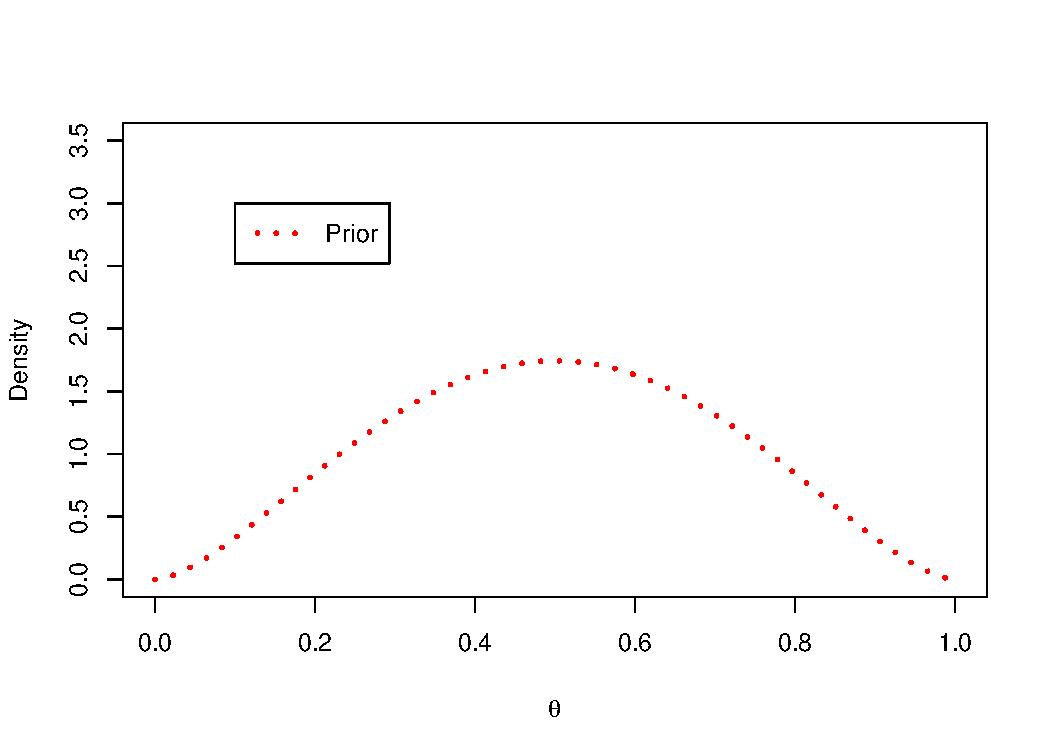
\includegraphics[width=.9\textwidth]{obama_prior.pdf}
\end{center}
}

\frame{

\begin{center}
\includegraphics[width=.9\textwidth]{obama_likprior.pdf}
\end{center}
}


\frame{
\begin{center}
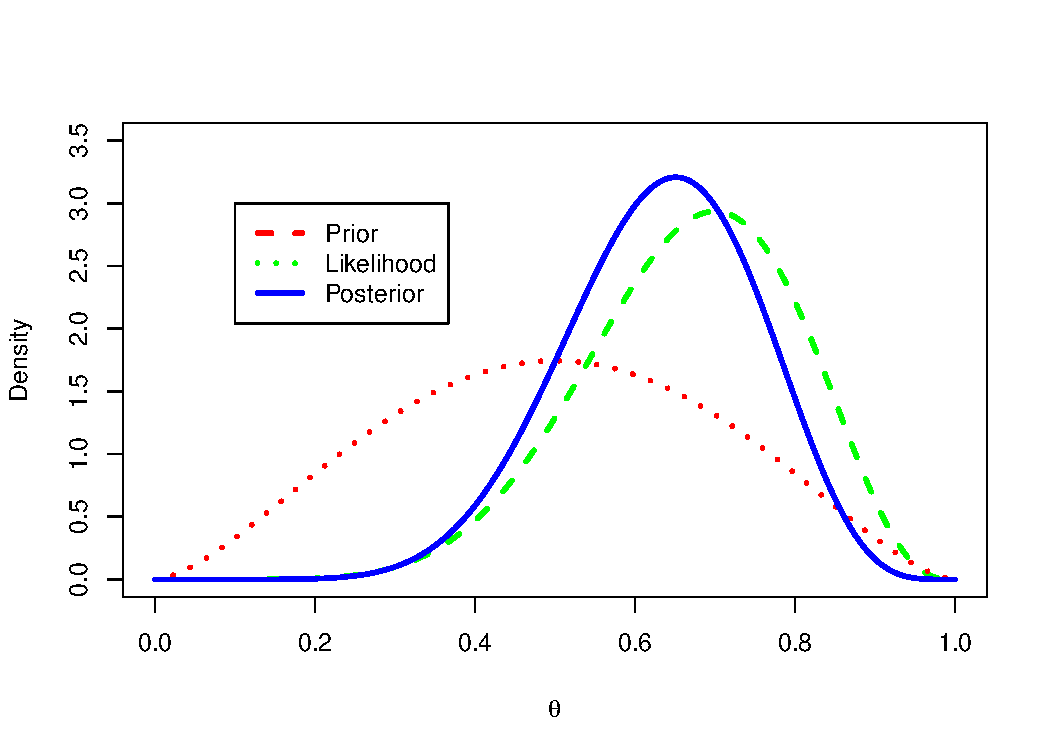
\includegraphics[width=.9\textwidth]{obama_all.pdf}
\end{center}
}

\section{History}

%\section{Advantages of Bayesian Methods}
\frame{


The basic philosophical difference between the frequentist and Bayesian paradigms is that 
\begin{itemize}
\item Bayesians treat an unknown parameter~$\theta$ as \emph{random}.
%and use probability to quantify their uncertainty about it.
\pause  
\item Frequentists treat $\theta$ as unknown but \emph{fixed}.
%and they therefore believe that probability statements about $\theta$ are useless.  
\end{itemize}

%This fundamental disagreement leads to entirely different ways to handle statistical problems, even problems that might at first seem very basic.
}



\section{Only the Likelihood Matters!}

\frame{
\frametitle{Stopping Rule}
Let $\tth$ be the probability of a particular coin landing on
heads, and suppose we want to test the hypotheses
\pause
$$H_0 : \tth = 1/2,\qquad H_1 : \tth > 1/2$$
at a significance level of $\alpha=0.05$.
Suppose we observe the following sequence of flips:
$$\text{heads, heads, heads, heads, heads, \textbf{tails}}\qquad\text{(5 heads, 1 tails)}$$
\pause
\begin{itemize}
\item To perform a frequentist hypothesis test, we must define a random variable to describe the data.  
\pause
\item The proper way to do this depends on exactly which of the following two experiments was actually performed:
\end{itemize}
}

\frame{
\begin{itemize}
\item Suppose the experiment is ``\textbf{Flip six times and record the results.}''  
\pause
\begin{itemize}
\item $X$ counts the number of heads, and $X\sim\text{Binomial}(6,\theta)$.  
\item The observed data was $x=5$, and the p-value of our hypothesis test is
\end{itemize}
\begin{eqnarray*}
\pause
\text{p-value}&=&P_{\theta=1/2}(X\ge5)\\
&=&P_{\theta=1/2}(X=5)+P_{\theta=1/2}(X=6)\\
\pause
&=&\frac{6}{64}+\frac{1}{64}=\frac{7}{64}=0.109375>0.05.
\end{eqnarray*}
\pause
\textbf{So we fail to reject} $H_0$ at $\alpha=0.05$.
\end{itemize}
}

\frame{

\begin{itemize}
\item Suppose now the experiment is ``\textbf{Flip until we get tails.}'' \\ 
\pause
\begin{itemize}
\item $X$ counts the number of the flip on which the first tails occurs, and $X\sim\text{Geometric}(1-\theta)$. 
\item  The observed data was $x=6$, and the p-value of our hypothesis test is
\end{itemize}
\begin{eqnarray*}
\text{p-value}&=&P_{\theta=1/2}(X\ge6)\\
\pause
&=&1-P_{\theta=1/2}(X<6)\\
\pause
&=&1-\sum_{x=1}^5P_{\theta=1/2}(X=x)\\
\pause
&=&1-\left(\frac{1}{2}+\frac{1}{4}+\frac{1}{8}+\frac{1}{16}+\frac{1}{32}\right)
=\frac{1}{32}=0.03125<0.05.
\end{eqnarray*}
\textbf{So we reject} $H_0$ at $\alpha=0.05$.
\end{itemize}

}
\frame{
\begin{itemize}
\item The conclusions differ, which seems strikes \emph{some people} as absurd.  
\pause
\item P-values aren't close---one is 3.5 times as large as the other.  
\pause
\item The result our hypothesis test depends on whether we would have stopped flipping if we had gotten a tails sooner. 
\pause
\item The tests are dependent on what we call the \emph{stopping rule}. 
%\item The frequentist approach requires us to specify what we would have done had the data been something that we already know it wasn't.
\end{itemize}
}

%\newpage
\frame{
\begin{itemize}
\item The likelihood for the actual value of $x$ that was observed is the same for both experiments (up to a constant):
$$p(x|\theta)\propto\theta^5(1-\theta).$$
\pause
\item A Bayesian approach would take the data into account only through this likelihood.
\pause
\item  This would  provide the same answers regardless of which experiment was being performed.
\end{itemize} 
\vspace*{1em}

%This is because the Bayesian analysis is independent of the stopping rule (think about how to show this at home). 

The Bayesian analysis is independent of the stopping rule since it only depends on the likelihood (show this at home!). 
}
%
%\begin{ex}
%Suppose we want to test whether the voltage~$\theta$ across some electrical component differs from 9~V, based on noisy readings of this voltage from a voltmeter.  Suppose the data is as follows:
%$$9.7,\; 9.4,\; 9.8,\; 8.7,\; 8.6$$
%A frequentist might assume that the voltage readings $X_i$ are iid from some $N(\theta,\sigma^2)$ distribution, which would lead to a basic one-sample $t$-test.
%
%However, the frequentist is then presented with an additional piece of information: 
%\textbf{The voltmeter used for the experiment only went up to 10~V, and any readings that might have otherwise been higher are instead truncated to that value.}  Notice that \emph{none of the voltages in the data are 10~V}.  In other words, we already know that the 10~V limit was completely irrelevant for the data we actually observed.
%
%Nevertheless, a frequentist must now redo the analysis and could perhaps obtain a different conclusion, because the 10~V limit changes the distribution of the observations under the null hypothesis.  Like in the last example, the frequentist results change based on what would have happened had the data been something that we already know it wasn't.
%\end{ex}
%
%The problems in Examples~1.1~and~1.2 arise from the way the frequentist paradigm forces itself to interpret probability.  Another familiar aspect of this problem is the awkward definition of ``confidence'' in frequentist confidence intervals.  
%
%\textbf{The most natural interpretation} of a 95\% confidence interval~$(L,U)$---that there is a 95\% chance that the parameter is between $L$ and $U$---\textbf{is dead wrong from the frequentist point of view.}  
%
%Instead, the notion of ``confidence'' must be interpreted in terms of repeating the experiment a large number of times (in principle, an infinite number), and no probabilistic statement can be made about \emph{this particualar} confidence interval computed from the data we actually observed.
%
%

\section{Hierarchical Bayesian Models}

\frame{
\frametitle{Hierarchical Bayesian Models}
In a hierarchical Bayesian model, rather than specifying the prior distribution as a single function, we specify it as a hierarchy. 
}
%Thus, on the unknown parameter of interest, say $\theta,$ we put a prior. On any other unknown \emph{hyperparameters} of the model that are given, we also specify priors for these. We write
\frame{
\frametitle{Hierarchical Bayesian Models}
\begin{align*}
X|\theta &\sim f(x|\theta) \\
\Theta|\gamma &\sim \pi(\theta|\gamma)\\
\Gamma &\sim \phi(\gamma),
\end{align*}
where we assume that $\phi(\gamma)$ is known and not dependent on any other unknown \emph{hyperparameters}. 
}

%Note that we can continue this hierarchical modeling and add more stages to the model, however note that doing so adds more complexity to the model (and possibly as we will see may result in a posterior that we cannot compute without the aid of numerical integration or MCMC, which we will cover in detail in a later chapter). 

\frame{
\frametitle{Conjugate Distributions}
Let $F$ be the class of sampling distributions $p(y|\theta).$ 
\pause
\begin{itemize}
\item Then let $P$ denote the class of prior distributions on~$\theta.$ 
\pause
\item Then $P$ is said to be conjugate to $F$ if for every $p(\theta) \in P$ and $p(y|\theta) \in F,$ $p(y|\theta) \in P.$
\end{itemize}
 \textbf{Simple definition}:
A family of priors such that, upon being multiplied by the likelihood,
yields a posterior in the same family. 
}

\begin{frame}

\frametitle{Beta-Binomial}
If $X|\tth$ is distributed as $\text{binomial} (n, \tth)$, then a conjugate prior
is the beta family of distributions, where we can show that the posterior is
\pause
\begin{eqnarray*}
%\begin{align*}
\pi(\theta|x) &\propto &  p(x|\theta)p(\theta)\\
\pause
& \propto  &
\binom{n}{x} \theta^x (1-\theta)^{n-x}
\frac{\Gamma(a + b)}{\Gamma(a)\Gamma(b)}
\theta^{a-1}(1-\theta)^{b-1} \\
\pause
&\propto &
 \theta^x (1-\theta)^{n-x} 
\theta^{a-1}(1-\theta)^{b-1} \\
\pause
& \propto &
 \theta^{x + a -1} (1-\theta)^{n-x + b-1} \implies
%\end{align*}
\end{eqnarray*}
\pause
$$\theta|x  \sim \text{Beta}(x+a,n- x +b).$$
\end{frame}


%\frame{
%
%\frametitle{Gamma-InverseGamma}
%%
%%\begin{ex}
%%\label{gamma}
%\begin{eqnarray*}
%X|\alpha,\beta &\sim& \text{Gamma}(\alpha,\beta),\; \alpha \;\text{known},\;\beta\; \text{unknown}\\
%\beta &\sim& \text{IG}(a,b).
%\end{eqnarray*}
%\pause
%%\end{ex}
%Calculate the posterior distribution of $\beta|x.$
%\begin{eqnarray*}
%p(\beta|x) &\propto& \frac{1}{\Gamma{(\alpha)}\beta^\alpha}x^{\alpha-1}e^{-x/\beta}\times
%\frac{b^a}{\Gamma{(a)}}\beta^{-a-1}e^{-b/\beta}\\
%\pause
%&\propto& \frac{1}{\beta^\alpha}e^{-x/\beta}
%\beta^{-a-1}e^{-b/\beta}\\
%\pause
%&=&\beta^{-\alpha-a-1}e^{-(x+b)/\beta} \implies
%\end{eqnarray*}
%%Notice that this looks like an Inverse Gamma distribution with parameters $\alpha + a$ and $x+b.$ Thus,
%$$\beta|x \sim IG(\alpha + a, x+b).$$
%}


\frame{
\frametitle{How Much Do You Sleep}
We are interested in a population of American college students and the proportion of the population that sleep at least eight hours a night, which we denote by $\theta.$
}

\frame{
\frametitle{Prior Data}
\begin{itemize}

\item  \emph{The Gamecock}, at the USC printed an internet article ``College Students Don't Get Enough Sleep" (2004).  \begin{itemize}
\item Most students spend six hours sleeping each night. 
\end{itemize}
\item 2003: University of Notre Dame's paper, \emph{Fresh Writing}. 
\begin{itemize}
\item The article  reported took random sample of 100 students:
\item ``approximately 70\% reported to receiving only five to six hours of sleep on the weekdays, 
\item 28\% receiving seven to eight, 
\item and only 2\% receiving the healthy nine hours for teenagers."
\end{itemize}
\end{itemize}
}

\begin{frame}[fragile]
\begin{itemize}
\item  Have a random sample of 27 students is taken from UF. 
\item 11 students record that they sleep at least eight hours each night. \item Based on this information, we are interested in estimating $\theta.$ 
\end{itemize}
\end{frame}

\frame{


\begin{itemize}

\item From USC and UND,  believe it's probably true that most college students get  \textcolor{red}{less than eight hours of sleep}. 
\item Want our prior to assign most of the probability to values of $\theta < 0.5. $
\item From the information given, we decide that our best guess for $\theta$ is 0.3, although we think it is very possible that $\theta$ could be any value in $[0,0.5].$
\end{itemize}
}

\frame{
\begin{itemize}
\item Given this information, we believe that the median of $\theta$ is $0.3$ and the $90$th percentile is 0.5. 
\item Knowing this allows us to estimate the unknown values of $a$ and $b$. 
\item After some calculations we find that $a = 3.3$ and $b = 7.2.$ How did we actually calculate $a$ and $b$?
\end{itemize}
\pause

We would need to solve the following equations:

$$\int_{0}^{0.3} \frac{\Gamma(a+b)}{\Gamma(a)\Gamma(b)}
\theta^{a-1}(1-\theta)^{b-1}\;d\theta = 0.5$$
$$\int_{0}^{0.5} \frac{\Gamma(a+b)}{\Gamma(a)\Gamma(b)}
\theta^{a-1}(1-\theta)^{b-1}\;d\theta = 0.9$$


}

\frame{
\begin{itemize}
\item In non-calculus language, this means the 0.5 quantile (50th percentile)~=~0.3. The 0.9 quantile (90th percentile) = 0.5. 
\item We can easily solve this numerically in \texttt{R} using a numerical solver \texttt{BBsolve}. 
\end{itemize}

Since you won't have used this command before, you'll need to install the package \texttt{BB} and load the library.

}

\begin{frame}[fragile]

Here is the code in \texttt{R} to find $a$ and $b$.

\begin{verbatim}
## install the BBsolve package
install.packages("BB", repos="http://cran.r-project.org")
library(BB)
fn = function(x){qbeta(c(0.5,0.9),x[1],x[2])-c(0.3,0.5)}
BBsolve(c(1,1),fn)

## alternative way
myfn <- function(shape){
	test <- pbeta(q = c(0.3, 0.5), shape1 = shape[1], 
	 shape2 = shape[2]) - c(0.5, 0.9)
	return(test)
	}
BBsolve(c(1,1), myfn)
\end{verbatim}
\end{frame}

%\texttt{BBsolve} is a numerical solver. You give it two arguments. First, you give it a set of initial values as your best guess of $a$ and $b$. Then you define a function which must take arguments as vectors for the unknown values of $a$ and $b$. The solver sets the function to zero and then finds the best solutions for $a$ and $b$ (we won't go into the details of how it solves for the values in this class). 
%
%So, in place of $a$ and $b$, we use $x[1]$ and $x[2]$ in our function (since it requires vectors). We also use the \texttt{qbeta} command because we're interested in the 0.5 and 0.9 quantiles. We must subtract 0.3 and 0.5 from each respective quantile since \texttt{BBsolve} sets our function to zero and solves. To do all of this in one step, we represent everything as a vector using \texttt{c()}. For example, \texttt{c(0.3,0.5)} represents the vector with elements 0.3 and 0.5. 
%
%If you have more questions on \texttt{function} or \texttt{BBsolve} remember you can get help by \texttt{?function} or \texttt{?BBsolve}.
\frame{

Using our calculations from the Beta-Binomial our model is
\begin{align*}
X \mid \theta &\sim \textrm{Binomial}(27,\theta)\\
\theta &\sim \textrm{Beta}(3.3,7.2)\\
\theta \mid x &\sim \textrm{Beta}(x+3.3,27-x+7.2)\\
\theta \mid 11 &\sim \textrm{Beta}(14.3,23.2)\\
\end{align*}
}
%
%\frame{
%We can easily plot the likelihood, prior, and posterior in R. The command \texttt{seq} below creates a sequence of 500 numbers between 0 and 1. Using the \texttt{plot} command, we plot the posterior distribution using \texttt{lty} (line type) 2 and \texttt{lwd} (line width) 3. For the \texttt{xlab} (x-label), we use \texttt{expression(theta)} so that a $\theta$ will print on the x-axis. The command \texttt{lines} allows us to add more plots onto the original plot. The \texttt{legend} creates a legend which is mostly straightforward. From Figure \ref{fig:sleep}, we can see that the posterior is a mixture of the likelihood and the prior. By visual inspection, the posterior mean appears to be around 0.4. We will come back to this example later to analyze other questions of interest.
%}

\begin{frame}[fragile]

\begin{verbatim}
th = seq(0,1,length=500)
a = 3.3
b = 7.2
n = 27
x = 11
prior = dbeta(th,a,b)
like = dbeta(th,x+1,n-x+1)
post = dbeta(th,x+a,n-x+b)
pdf("sleep.pdf",width=7,height=5)
plot(th,post,type="l",ylab="Density",lty=2,lwd=3,
xlab = expression(theta))
lines(th,like,lty=1,lwd=3)
lines(th,prior,lty=3,lwd=3)
legend(0.7,4,c("Prior","Likelihood","Posterior"),
lty=c(3,1,2),lwd=c(3,3,3))
dev.off()
\end{verbatim}
\end{frame}

\begin{figure}[h]
\centering
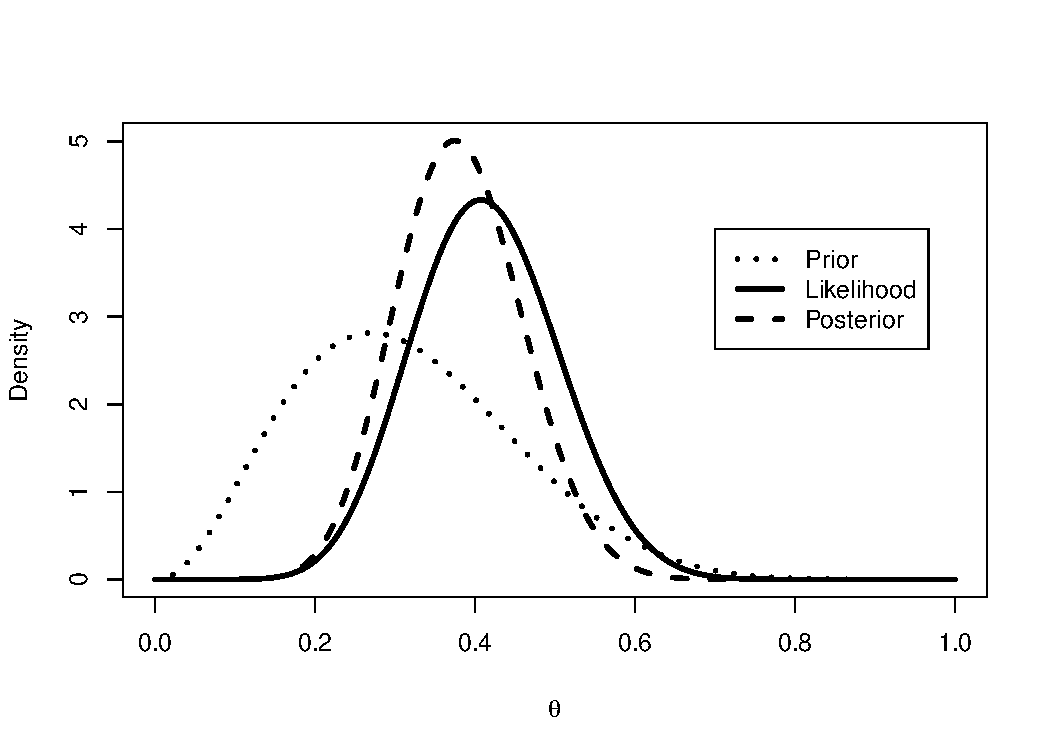
\includegraphics[width = .7\textwidth]{sleep.pdf}
\caption{Likelihood $p(X|\theta)$ , Prior $p(\theta)$, and Posterior Distribution $p(\theta|X)$}
\label{fig:sleep}
\end{figure}


}

\end{frame}

%\frame{
%\frametitle{Multivariate Distributions}
%\begin{eqnarray*}
%\bX\mid \tth &\sim& N(\tth, \Sigma) \\ 
%\tth &\sim& N( \bmu, \Omega)
%\end{eqnarray*}
%\begin{eqnarray*}
%\pi(\tth \mid \bx ) & \propto &
%\exp\{ -1/2||\bx - \tth ||_\Sigma\}
%\exp\{ -1/2||\tth - \bmu ||_\Omega\}.
%\end{eqnarray*}

%Note that
%\begin{eqnarray*}
%&& (\bx - \tth)^T\Sigma^{-1} (\bx - \tth) 
%+ 
%(\tth - \bmu)^T\Omega^{-1} ( \tth -\bmu)  \\
%&=&
%\bx^T\Sigma^{-1} \bx
%+ \bmu^T\Omega^{-1} \bmu 
%+ \tth^T\Sigma^{-1}\tth -2\bx^T\Sigma^{-1}\tth +\bth^T\Omega^{-1} \bth \\
%&+&\bmu \Simga^{-1} \bmu - 2 \bmu^T \Sigma^{-1} \bth
%\end{eqnarray*}




}
%
%\frame{
%
%\begin{eqnarray*}
%\pi(\tth \mid \bx ) & \propto &
%\exp\{ -1/2||\bx - \tth ||_\Sigma\}
%\exp\{ -1/2||\tth - \bmu ||_\Omega\}.
%\end{eqnarray*}
%
%Note that
%\begin{eqnarray*}
%&& (\bx - \tth)^T\Sigma^{-1} (\bx - \tth) 
%+ 
%(\tth - \bmu)^T\Omega^{-1} ( \tth -\bmu)  \\
%\pause
%&=&
%\bx^T\Sigma^{-1} \bx
%+ \bmu^T\Omega^{-1} \bmu 
%+ \tth^T\Sigma^{-1}\tth -2\bx^T\Sigma^{-1}\tth +\tth^T\Omega^{-1} \tth \\
%\pause
%&+&\bmu \Sigma^{-1} \bmu - 2 \bmu^T \Sigma^{-1} \tth \\
%\pause
%&\propto& 
% \tth^T\Sigma^{-1}\tth -2\bx^T\Sigma^{-1}\tth +\tth^T\Omega^{-1} \tth 
% - 2 \bmu^T \Sigma^{-1} \tth \\
% \pause
% &\propto& \left\{ \tth - (\Sigma^{-1}+ \Omega^{-1})^{-1} \left(
% \Sigma^{-1}\bx+ \Omega^{-1}\tth
% \right)
% \right\}^T \times
% (\Sigma^{-1}+ \Omega^{-1})^{-1} \\
% \pause
% &\times&
% \left\{
%  \tth - (\Sigma^{-1}+ \Omega^{-1})^{-1} \left(
% \Sigma^{-1}\bx+ \Omega^{-1}\tth
% \right)
% \right\}  \impies
%\end{eqnarray*}
%$$\tth \mid \bx \sim N\left( (\Sigma^{-1}+ \Omega^{-1})^{-1} \left(
% \Sigma^{-1}\bx+ \Omega^{-1}\tth
% \right), 
%  (\Sigma^{-1}+ \Omega^{-1})^{-1} 
%\right )$$
%
%
%
%
%
%
%}


%%Next time: Gibbs sampling. For more complicated model, we can not calculate the posterior in closed form, we must estimate it. How can we do this? 






\end{document}